\documentclass{article}
\usepackage{ctex}
\usepackage{graphicx}
\usepackage{amsmath}
\usepackage{indentfirst}
\usepackage{titlesec}
\usepackage{setspace}
\usepackage{subfigure}
\usepackage{caption}
\usepackage{float}
\usepackage{booktabs}
\usepackage{geometry}
\usepackage{multirow}
\usepackage{hyperref}
\hypersetup{
	colorlinks=true,
	linkcolor=blue,
	filecolor=magenta,      
	urlcolor=cyan,
	pdftitle={Overleaf Example},
	pdfpagemode=FullScreen,
}
\geometry{left=1.2cm,right=1.2cm,top=2cm,bottom=2cm}
\title{\songti \zihao{2}\bfseries HW7 Romberg算法}
\titleformat*{\section}{\songti\zihao{4}\bfseries}
\titleformat*{\subsection}{\songti\zihao{5}\bfseries}
\renewcommand\thesection{\arabic{section}}
\author{王启骅 PB20020580}
\begin{document}
	\maketitle
	\section{算法描述}
	首先定义函数vx,vy,参数为t(时刻),M(最大迭代数),采用Romberg积分算法求解t时刻的速度。从区间左端点a=0积分到区间右端点b=t,分别对$ a_x,a_y $积分,分割区间h=$ \frac{t}{n}=t $,积分流程与课本相同,首先求得k=1情况
	\begin{equation}
		R_{1,1}=\frac{a(0)+a(t)}{2}h
	\end{equation}
其中a代表x或y方向加速度。


接下来求解当k>1时,利用递推式求解。首先取h=$ \frac{h}{2} $作为本次迭代得区间划分长度h值。对于k=2-M
\begin{equation}
	R_{k,1}=\frac{R_{k-1,1}+2h\sum_{i=1}^{2^{k-2}}a(0+(2i-1)h)}{2}
\end{equation}
对于j=2-k
\begin{equation}
	R_{k,j}=R_{k,j-1}+\frac{R_{k,j-1}-R_{k-1,j-1}}{4^{j-1}-1}
\end{equation}
当循环到$ |R_{k,k}-R{k-1,k-1}|<e $时退出循环。


在这里的计算中,为了节省内存,取了$ 2\times M $的数组R,并且取了count=0,对于每次循环,通过count的奇偶来判断R[0]或R[1]作为本次赋值对象,即用count对2取模来实现。每次循环结束count=count+1 。最后输出$ R_{k,k} $即为在t时刻点的速度。


对于x,y坐标点的求解采用完全相同的算法,只是将以上积分过程中的$ a_x,a_y $函数替换为$ v_x,v_y$,这里不再赘述。
	\section{结果与讨论}
在M=8情况下,计算得到的轨迹图如图\ref{fig:1}
\begin{figure}[!h]
	
	\centering
	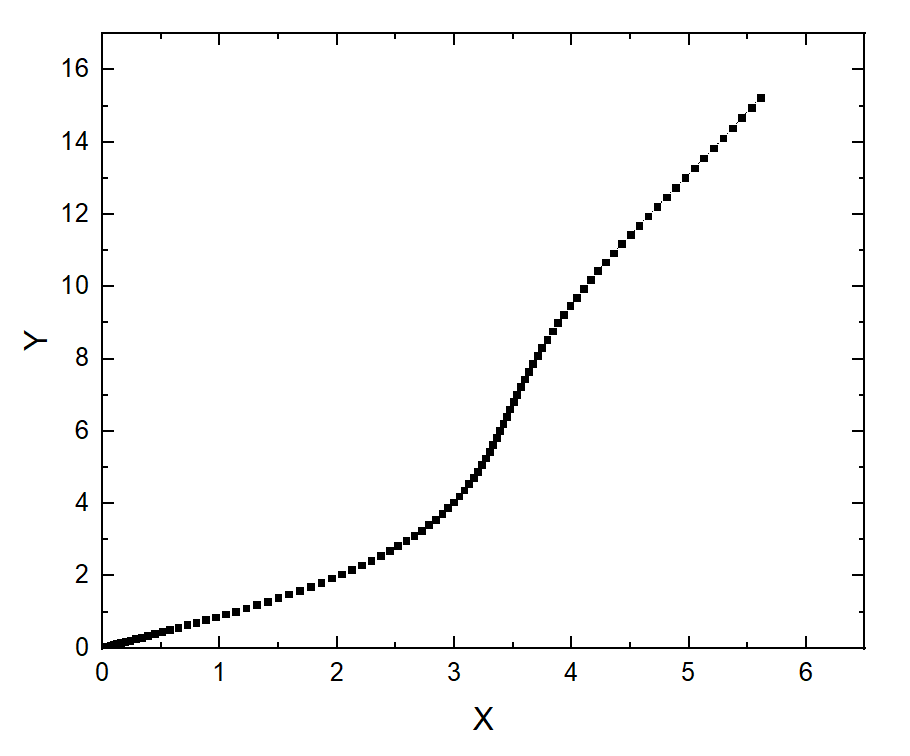
\includegraphics[scale=0.8]{track}
	\captionsetup{font={small},labelfont=bf}
	\caption{\heiti\zihao{-5}轨迹图}
	\label{fig:1}
\end{figure}
	
	
	计算达到精度的比例如图\ref{fig:2}
	\begin{figure}[!h]
		
		\centering
		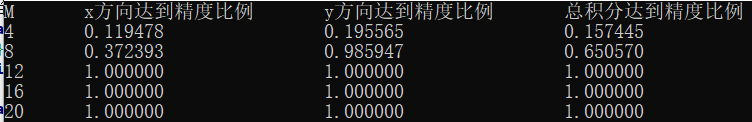
\includegraphics[scale=1.0]{error}
		\captionsetup{font={small},labelfont=bf}
		\caption{\heiti\zihao{-5}达到精度的比例}
		\label{fig:2}
	\end{figure}
在M=4-8时比例迅速增长,总比例从0.157445增长到0.650570 。而到了M=12后比例以达到1,说明已经全部达到精度。但是根据对x,y方向分别的讨论,可以看出对于不同的函数,积分达到精度的情况是不同的,y方向收敛速度明显快于x方向。M是在总体上起到对精度和计算效率的调控的作用,在使迭代能尽量达到精度的情况下,又防止某一特定点迭代所需次数过多而计算速率过慢。所以我们在进行实际运算中,需要根据对于计算的精度、效率双重考虑,取恰当的M值使在能够达到需要精度的前提下尽量快速的完成。而且要根据函数的不同,相应的迭代收敛速度也不同,选取不同的M。
\end{document}